\documentclass[a4paper,12pt]{article}
\usepackage{graphicx}
\begin{document}

In this part, upon the two-ubuntu LAN that we built previously, we use FTP (File transfer protocol) to transfer a 7353 bytes file from host to server. And using Wireshark, I will give a detailed analysis on how the ftp files break into packets and into bits.

\begin{figure}[ht!]
\centering
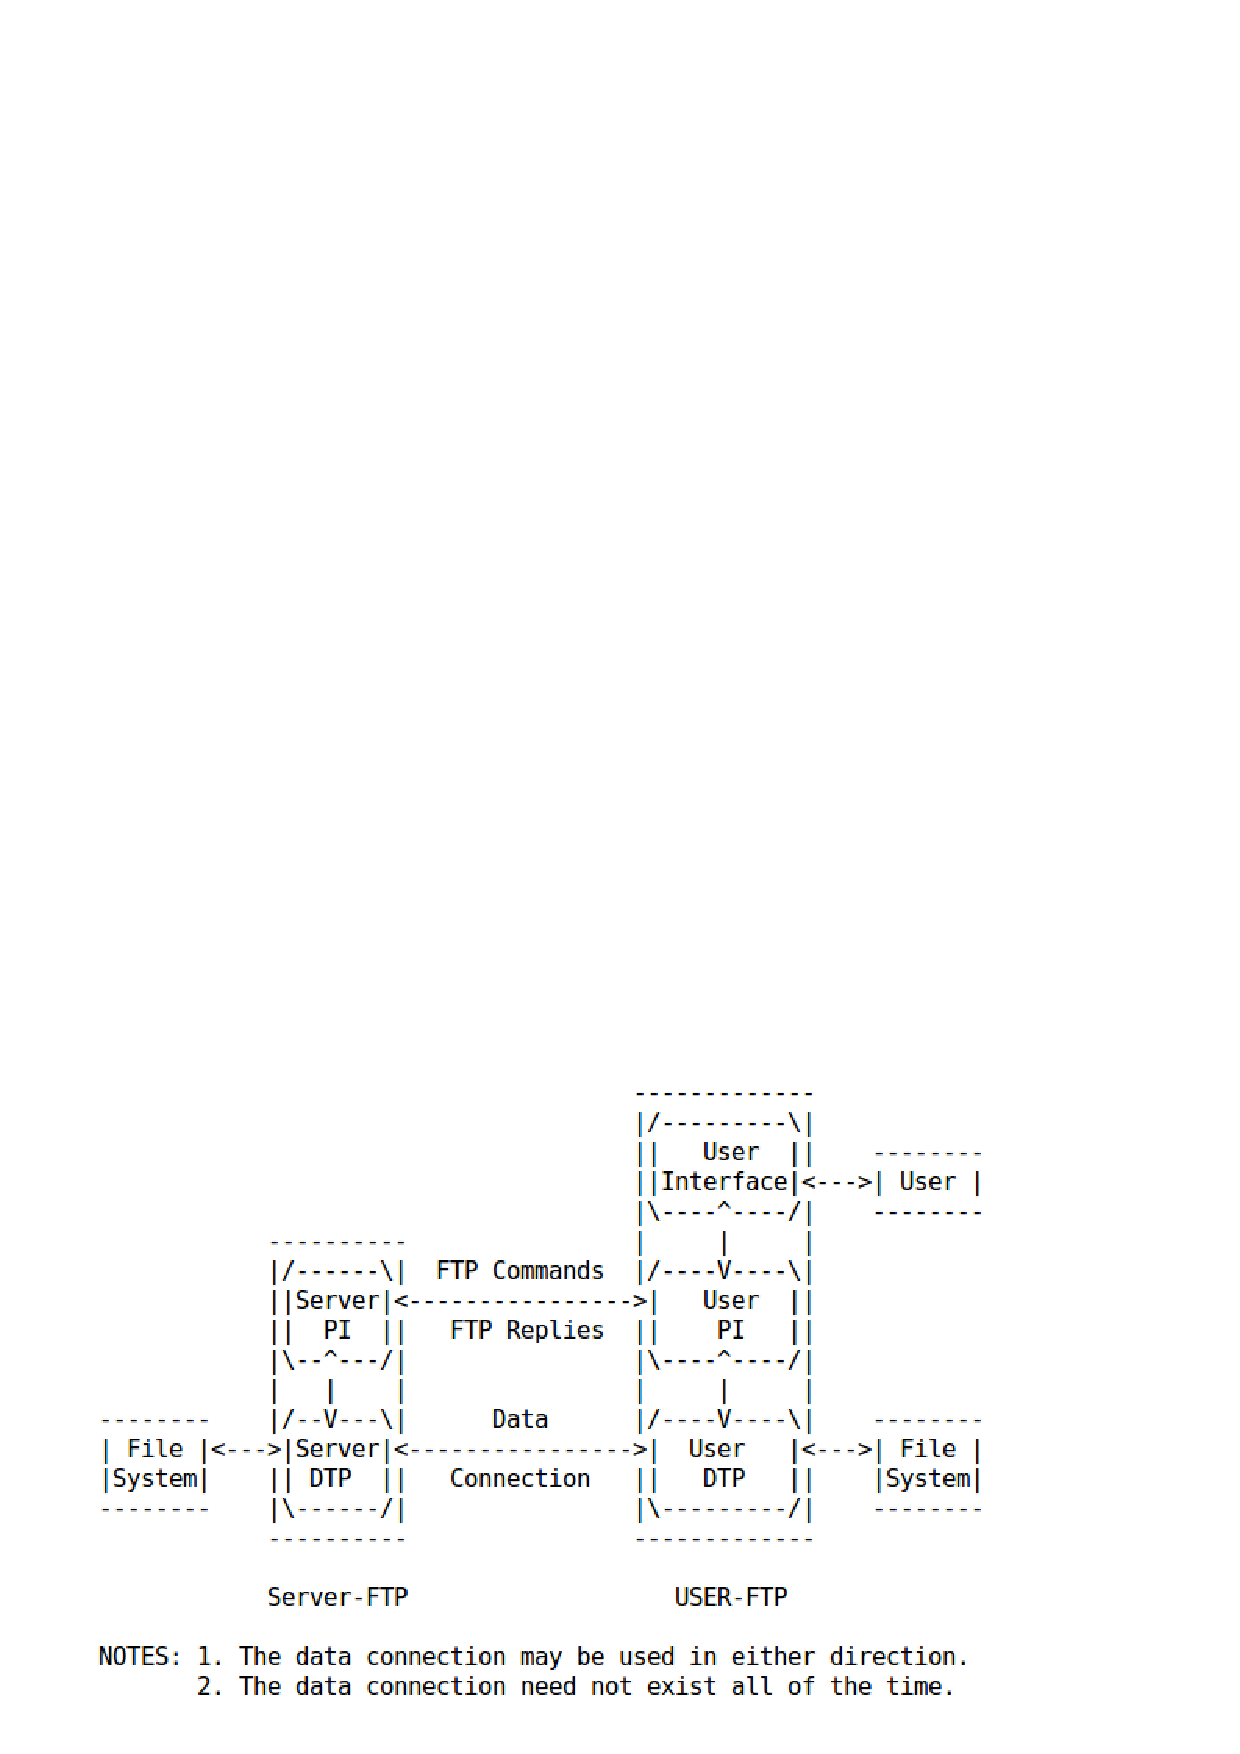
\includegraphics[width=120mm]{ftp-model.png}
\caption{1 \label{overflow}}
\end{figure}

As can be seen from this picture, the data connection is established between the server DTP (data transfer process) and the user DTP, as for ftp commands and replies, they are transfered between server PI (protocol interpreter) and user PI.

\begin{figure}[ht!]
\centering
\includegraphics[width=120mm]{1.png}
\caption{2 \label{overflow}}
\end{figure}

The above figure shows a typical ftp data connection establishment. 
1, host request server for connection.
2, server responses code 200, meaning that connection permmitted.
3, and port 179,6 (45830) is to be used
4, use PASV, a mode where the client initiates the data connection.
5, ready to return the aimed file Annotator.java.

\begin{figure}[ht!]
\centering
\includegraphics[width=120mm]{2.png}
\caption{3 \label{overflow}}
\end{figure}

This image is a typical 3-way-hand-shaking TCP, to synthesize and establish a reliable connection.

\begin{figure}[ht!]
\centering
\includegraphics[width=120mm]{3.png}
\caption{4 \label{overflow}}
\end{figure}

This image shows that, code 150 means "File status okay; about to open data connection."

\begin{figure}[ht!]
\centering
\includegraphics[width=120mm]{4.png}
\caption{5 \label{overflow}}
\end{figure}

Finally, we come to the file transfers, we can see that the files are transferred in several parts, and after each part of data transferred into user, user would send an ACK (acknowledgement) back to server, meaning that the user received the data successfully. At the end, code 226 means "Closing data connection. Requested file action successful (for example, file transfer or file abort)."

\begin{figure}[ht!]
\centering
\includegraphics[width=120mm]{5.png}
\caption{6 \label{overflow}}
\end{figure}

Figure 6 shows one of the ftp-data packet, where bits of the packet can be seen.

First, how can we know if the packet is the ftp-data packet? We can check the source port (20 as ftp data) and destination port, and in the meantime check if there are bits after 66 bytes. (We will see the code inplementation of this soon)

Thus, similarly, for every ftp-data packet, we can grab those bits of data from the 66 bytes of the packet to the end.

Now let's look into the bits of one of the ftp-data packet of the file (Annotator.java). 

\begin{figure}[ht!]
\centering
\includegraphics[width=120mm]{6.png}
\caption{7 \label{overflow}}
\end{figure}

For each packet:

\begin{figure}[ht!]
\centering
\includegraphics[width=120mm]{7.png}
\caption{8 \label{overflow}}
\end{figure}

1, first 6 bytes (0~5) are user mac address(d4:be:d9:50:fa:b2 here), 6~11 (6) bytes are server mac address (40:3c:fc:01:04:85), 12~13 (2) bytes are IP (0X0800). 

\begin{figure}[ht!]
\centering
\includegraphics[width=120mm]{8.png}
\caption{9 \label{overflow}}
\end{figure}

2, 14 byte is header length (20), ignore 15 byte, 16~17 (2) bytes are total length of data transferred (1500), 18~19 (2) bytes are identification (0x2fcb -> 12235), 20~21 (2) bytes are fragment offset (0), 22 is time to live (64), 23 byte is protocol used (6 -> TCP), 24~25 (2) bytes are header checksum (0x81f5 -> validation disabled), 26~29 (4) bytes are source GeoIP (unknown), 30~33 (4) bytes are destination GeoIP (unknown).

\begin{figure}[ht!]
\centering
\includegraphics[width=120mm]{9.png}
\caption{10 \label{overflow}}
\end{figure}

3, 34~35 (2) bytes are source port (20 -> ftp-data port), 36~37 (2) bytes are destination port (45830), 38~41 (4) bytes are sequence number (1), 42~45 (4) bytes are acknowledgment number (1), 46~47 (2) bytes are flags (0x010), 
48~49 (2) bytes are window size value and scaling factor, 50~51 (2) bytes are checksum (0x7ab7 -> validation disabled), and the rest bytes all belong to TCP, until 62~65 (4) bytes are timestamp echo reply (279682).

4, then we see our data (1448 bytes), which takes a large part of the packet.

Thus, this analysis gives us the hint of how to abstract the bits of the file out of the packets flow.

\end{document}
